\documentclass[conference]{IEEEtran}
\IEEEoverridecommandlockouts
% The preceding line is only needed to identify funding in the first footnote. If that is unneeded, please comment it out.
\usepackage{cite}
\usepackage{amsmath,amssymb,amsfonts}
\usepackage{algorithmic}
\usepackage{graphicx}
\usepackage{textcomp}
\usepackage{xcolor}
\def\BibTeX{{\rm B\kern-.05em{\sc i\kern-.025em b}\kern-.08em
    T\kern-.1667em\lower.7ex\hbox{E}\kern-.125emX}}
\begin{document}

% --- TITLE ---
\title{Attention-Guided YOLOv11 for Object Detection in Unstructured Bangladeshi Traffic}

\maketitle

\begin{abstract}
In South Asian context, traffic is complex and chaotic due to its high population, unstructured roads, and various types of transport. Vision-based systems face massive challenges here due to extreme visual occlusion, a wide variety of unpredictable vehicle shapes, and erratic environments. Common standard real-time object detection models are mostly trained on structured datasets from developed countries, which fail to generalize to our region. This makes them less useful for Advanced Driver Assistance Systems (ADAS). We propose a modified YOLOv11 architecture integrated with attention modules capable of handling complex backgrounds and dense traffic. Our model uses Convolutional Block Attention Module (CBAM) injected specifically into the P5 feature map to improve core feature extraction capabilities in these complex environments. To train the model, we curated a custom dataset of over 265,000 annotated instances sourced from the Mendeley Bangladeshi Traffic Flow Dataset to focus on nonstandard local vehicles like rickshaws and CNG based on our region. Our ablation study in 50 epoch shows that baseline YOLOv11m achieved 75.1\% mAP while the optimized CBAM model improved performance to 75.7\% mAP on the validation set, maintaining real-time inference(~4.7 ms/frame). The attention mechanism excelled over the complex vehicle by outperformed the Rickshaw class with 90.8\% mAP and boosting truck detection by 1.5\%. Error analysis reveals architecture is highly sensitive to extreme data imbalance, especially for minority classes like cycles. We did a detailed qualitative ablation study and checked the confusion matrix which finds that changing the network architecture helps stabilize the system but lack of data is main bottleneck for detecting minority classes in intelligent transportation networks.
\end{abstract}

\begin{IEEEkeywords}
Object Detection, YOLOv11, Convolutional Block Attention Module, Advanced Driver Assistance Systems, Unstructured Traffic, Deep Learning.
\end{IEEEkeywords}

\section{Introduction}
In the modern era, transportation system lean towards (ITS) Intelligent Transportation Systems and (ADAS) Advanced Driver Assistance Systems which require real-time cameras and object detectors. Standard Western datasets like KITTI\cite{1a}, Cityscapes\cite{2a}, or COCO\cite{3a} fail to represent the reality of Dhaka traffic due to messy environment, different vehicle shapes and density, unpredictable pedestrians, unstructured streets and vehicles constantly blocking each other from the camera's view. Road is not only the challenges here, non-motorized and custom-built vehicles like rickshaws, CNGs, auto-rickshaws, easy-bikes, vans, etc causes trouble and don't exist in standard datasets \cite{Hasan2021VehicleClassification}. To give driver a reliable collision warning as ADAS, the system has to recognize these specific shapes first but all the previous models never seen them so they struggle to detect them. Another challenge is in dense traffic from the camera view multiple car overlap or hide behind one another which means the full detectable shape is not visible so when standard Non-Maximum Suppression (NMS) algorithms try to process these they usually delete valid bounding boxes by assumes that two overlapping vehicles are just a duplicate detection of a single car, rather than two separate vehicles. We tackle exactly these problems to detect overlapping objects clutter by its Convolutional Block Attention Module (CBAM)\cite{Woo2018CBAM} which guide the network to focus on the important structural edges of the vehicles in complex scene. We curated the Bangladeshi Traffic Flow Dataset from Mendeley Data\cite{Islam2025BangladeshiTrafficFlow} to focus on local vehicles. The results achieved a remarkable 90.8\% mAP@50, particularly for the visually complex vehicle class Rickshaw on Bangladeshi roads.
Overall, our main contributions are:
\begin{enumerate}
    \item We curated and standardized a custom dataset from local traffic images and annotating regional vehicles for complex Bangladeshi traffic.
    \item We proposed a modified YOLOv11m architecture that injects CBAM attention blocks into the deep layers to handle heavy occlusion.
    \item We thoroughly tested the model on edge-grade hardware to prove it can run in real-time.
    \item We did a deep qualitative failure analysis, isolating specific issues like confusing bicycles with people or trucks with buses. This proves that you cannot fix extreme data imbalance in developing regions just by changing the architecture.
\end{enumerate}
The paper reviews related work in Section II and Section III shows the proposed CBAM-integrated YOLOv11 architecture. Sections IV and VII cover the dataset, experimental setup, and performance analysis, and  Section VIII concluding remarks and future work.

\section{RELATED WORK}

\subsection{Evolution of Real-Time Object Detection}

For the past few years object detection rely on heavy, two-stage networks but everything changed when Redmon et al. introduced the original YOLO (You Only Look Once) architecture\cite{redmon2016you}. YOLO family evolved over the last few years rapidly with new versions and improvements. Recently, Jocher et al. advanced YOLO further with YOLOv11, reducing parameter counts\cite{Jocher2025YOLOv11}. Later on improving deep feature extraction through novel C3k2 modules and C2PSA attention mechanisms\cite{9a}. But yet fundamental challenge remains in YOLO architectures and it struggle with unstructured data. Zhang et al. observe in comparative studies that baseline YOLOv11 models face limitations in detecting highly occluded or structurally complex small objects\cite{zhang2025trinext}. When YOLOv11 is deployed in dense, overlapping clusters of vehicles then recall drops significantly because the baseline cannot separate highly occluded bounding boxes without architectural modification.

\subsection{Attention Mechanisms in Computer Vision}
When a neural network gets very deep it often loses fine details of small or partially hidden objects. To fix this issue, an attention mechanism was introduced to guide the network “where” and “what” to focus on such as the Squeeze-and-Excitation (SE) network by Hu et al., which effectively captured channel importance, but ignored spatial location information entirely \cite{11a}. To overcome this limitation, Woo et al. introduce (CBAM) Convolutional Block Attention Module \cite{Woo2018CBAM}, which achieves achieves better attention by applying channel attention first, then spatial attention sequentially. Recently, integration of CBAM into the YOLOv11 backbone has become a key research focus for handling complex environments. In July 2025, Garshasebi et al.\cite{garshasebi2025improving} integrated CBAM into YOLOv11 for remote sensing imagery which achieving a mean Average Precision (mAP@50) of 76.68\% by focusing on critical regions and reducing background noise. Also Khan et al. applied YOLOv11 with CBAM for pipeline defect detection and got accuracy improvements compared to the baseline model\cite{Rahman2021YOLOv5}. These studies prove CBAM is very effective at extracting weak geometric features from noisy backgrounds and highlights important features even when objects overlaping dense and overlapping scenes.

\subsection{Perception in Unstructured Traffic (The South Asian Context)}
When it comes to intelligent transportation in developing regions, the research is still catching up. In Bangladeshi perspective, traffic in cities like Dhaka, Gazipur is chaotic and unstructured which do not include native vehicles like rickshaws or CNGs in standard Western datasets. The challenges early attempts face is they struggled with unstructured traffic detection. For example, in 2021 study by Rahman et al.\cite{rahman2021densely} using an ensemble of YOLOv5 models on the Dhaka-AI dataset and reached mAP of only 45.8\% which shows the extreme difficulty of detecting traffic in such conditions. Recently, the open-source community has provided better datasets, such as the Bangladeshi Traffic Flow Dataset by Islam et al. \cite{Islam2025BangladeshiTrafficFlow}. In 2022, Rahman et al.\cite{rahman2022fine} fine-tuned deep convolutional networks to classify native Bangladeshi vehicles with improved accuracy. Hossain et al.\cite{17a} analyzed the conditions of rickshaw pullers in Dhaka city and highlighted the significant presence of non-motorized transport in urban traffic environments. Earlier studies usually treat deep learning models as black boxes, using transfer learning without fixing the mathematical cause of bounding box suppression in dense traffic. Our research differ from those earlier studies by building on regional datasets but go beyond simple retraining. We actively modify the YOLOv11 architecture instead of just applying transfer learning by injecting CBAM directly into the deep feature layers which target the extreme occlusion issues in South Asian traffic across a full, 9-class unstructured environment.

\section{MATHEMATICAL FORMULATION AND PROPOSED ARCHITECTURE}
We discovered several mathematical limits of the YOLOv11 in chaotic contexts by analyzing the baseline model. We tend to resolve these by introducing a spatial channel attention mechanism. 


\subsection{Baseline YOLOv11 Formulation}

YOLOv11 identifies objects in the images by predicting the position of objects by identifying the bounding boxes using learnt visual features. Nevertheless, it is difficult to detect in the most congested areas like Dhaka because of heavy traffic and obscuring objects, whereby cars usually come between the lens and the captured objects. In order to overcome this challenge, the base model uses Complete Intersection over Union (CIoU) loss that bounds box regression by taking into consideration the overlap, center distance, and aspect ratio consistency of the predicted and ground-truth boxes.. The CIoU loss is defined as:

\begin{equation}
L_{CIoU} = 1 - IoU + \frac{\rho^2(b, b_{gt})}{c^2} + \alpha \nu
\end{equation}


\subsection{Convolutional Block Attention Module (CBAM)}
The baseline model has a limitation during the deep feature extraction stage. When a bus occludes the lower part of a car, the feature extraction process may confuse the remaining visible features with background information, which can lead to missed detections. To address this issue, we incorporate the Convolutional Block Attention Module (CBAM)\cite{Woo2018CBAM}, which helps the model focus on more informative features..

CBAM forces the network to calculate "What is important?" (Channel Attention) and "Where is it?" (Spatial Attention). When an intermediate feature map $F \in \mathbb{R}^{C \times H \times W}$, CBAM sequentially generates a 1D channel attention map $M_{c}$ and a 2D spatial attention map $M_{s}$. The sequential attention process is formulated as:
\[
F' = M_{c}(F) \otimes F
\]
\[
F'' = M_{s}(F') \otimes F'
\]


(where $\otimes$ denotes element-wise multiplication).

\begin{enumerate}
    \item \textbf{Channel Attention:} At the channel attention stage, spatial information from the feature map is compressed using both average pooling and max pooling. These pooled features are then passed through a shared Multi-Layer Perceptron (MLP), which learns the importance of each channel.
    
    \item \textbf{Spatial Attention:} In the spatial attention stage, the channel-refined feature map $F'$ is first pooled along the channel dimension and then processed using a convolution layer with a $7 \times 7$ kernel. The larger receptive field allows the model to capture broader spatial relationships within the scene, and this approach helps the model to detect objects that are partially hidden, such as pedestrians standing close to large buses.

\end{enumerate}


\subsection{Architectural Integration Strategy}
Rather than adding the attention mechanism to the detection head, we designed a custom \texttt{ULTIMATE\_CBAM} module and injected it within the YOLOv11m backbone.

In our implementation, we replace the regular block at Layer~23 with a CBAM block. At this stage, the module receives the $P5$ feature map before the features are passed to the Detect head. In YOLOv11m, the width multiplier is set to $1.00$, so the $P5$ layer operates with $512$ channels. Passing this $512$-channel feature map through the CBAM module helps the network focus more on vehicle-related features while reducing less important background information.







\begin{figure}[h]
\centering
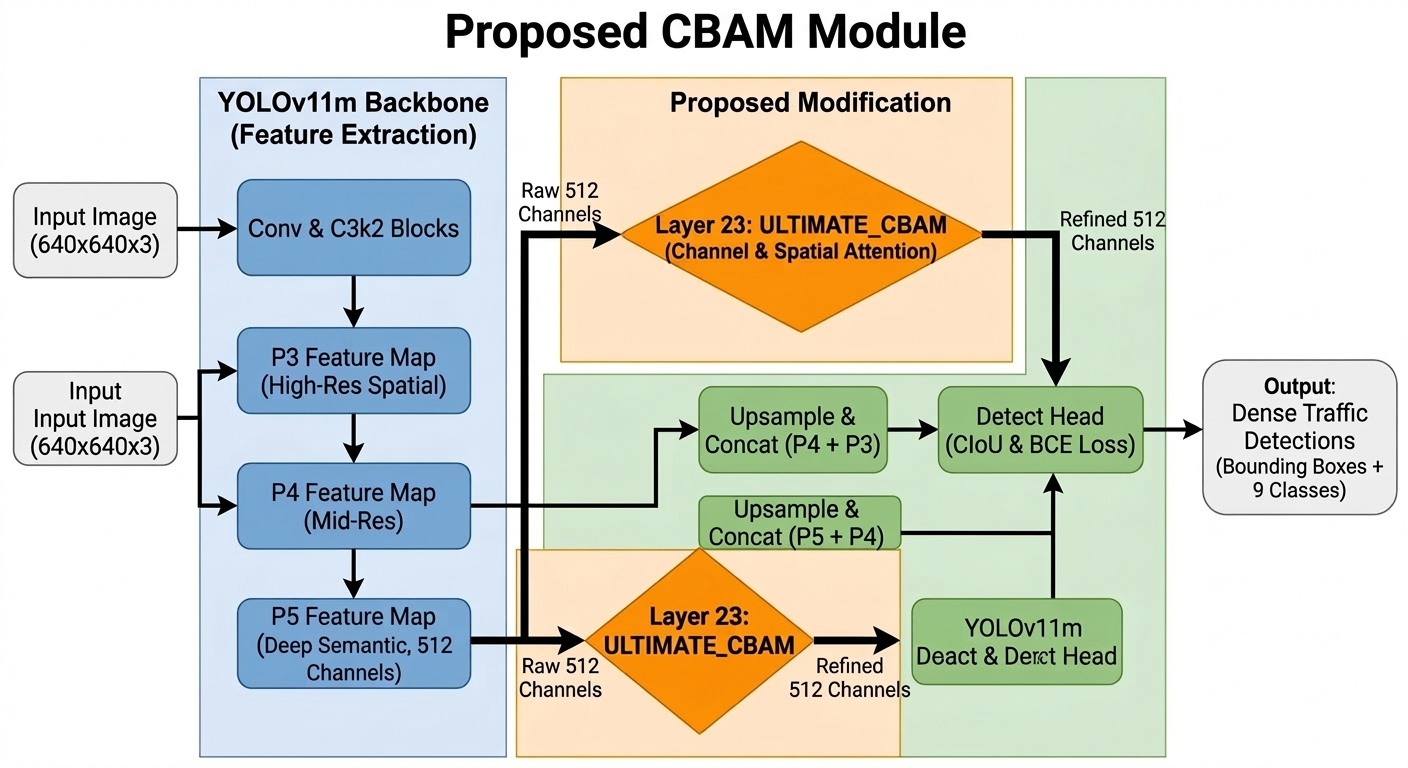
\includegraphics[width=0.9\linewidth]{Images/arch.png}
\caption{Proposed attention-guided YOLOv11m architecture. The standard feature extraction backbone is modified by injecting a Convolutional Block Attention Module (CBAM) specifically at Layer~23. This intercepts the 512-channel P5 feature map prior to the detection head, applying sequential channel and spatial attention to filter background noise and emphasize the structural edges of highly occluded vehicles.}
\label{fig:arch}
\end{figure}

\section{DATASET AND PREPROCESSING}
Collecting high-quality and properly annotated datasets is often challenging in many developing regions. Vehicles that are common in South Asian traffic, such as three-wheelers and various non-motorized transport, are rarely represented in widely used global datasets. For this reason, we created a custom dataset designed to reflect the real traffic conditions of Bangladesh in order to train our perception model.

\subsection{Data Sourcing and Curation}
We built our dataset by combining images collected from several regional traffic datasets. Most images collected from the Mendeley Bangladeshi Traffic Flow Dataset\cite{Islam2025BangladeshiTrafficFlow}. Extra images aded from the Dhaka-AI Dataset\cite{DVN/POREXF_2020} and Poribohon-BD Dataset\cite{19} to include more complex urban traffic scenes. Several preprocessing steps needed for the datasets before training the model. Few issues were annotations stored in XML and JSON formats and inconsistent bounding box coordinates in some subsets so we created a preprocessing script that parse annotations, clean incorrect values, and convert bounding box labels into normalized YOLO text format which makes a consistent dataset structure for training and evaluation. After preprocessing, the final dataset contains 23,648 images in total, including 18,919 images for training and 4,729 for validation. Across these images, we annotated 265,698 bounding boxes covering nine different vehicle classes commonly found in Bangladeshi traffic. To better understand how data availability affects model performance, we grouped the classes into three categories based on the number of instances in the dataset:

\begin{itemize}
    \item \textbf{Dominant Classes ($>$50,000 instances):} Car, Rickshaw, Bus
    \item \textbf{Mid-Tier Classes (10,000--50,000 instances):} People, CNG, Bike
    \item \textbf{Minority/Scarce Classes ($<$10,000 instances):} Mini-Truck, Truck, Cycle
\end{itemize}


The class distribution of the dataset is summarized in Table I. The numbers show a strong class imbalance in the collected traffic data. Vehicles such as cars and rickshaws appear far more frequently, while classes like cycles are much less common. In fact, the number of car instances is nearly 88 times higher than that of cycles.The class distribution of the dataset is summarized in Table I. The numbers show a strong class imbalance in the collected traffic data. Vehicles such as cars and rickshaws appear far more frequently, while classes like cycles are much less common. In fact, the number of car instances is nearly 88 times higher than that of cycles.

\begin{table}[htbp]
\caption{Distribution of Classes in the Finalized Dataset}
\centering
\resizebox{\linewidth}{!}{%
\begin{tabular}{|c|c|c|c|c|}
\hline
\textbf{Class Category} & \textbf{Vehicle Class} & \textbf{Train Instances} & \textbf{Validation Instances} & \textbf{Total Instances} \\
\hline
{Dominant} 
 & Car       & 50,584 & 12,523 & 63,107 \\
 & Rickshaw  & 48,357 & 11,884 & 60,241 \\
 & Bus       & 41,573 & 10,423 & 51,996 \\
\hline
{Mid-Tier} 
 & People    & 30,924 & 7,855  & 38,779 \\
 & CNG       & 22,356 & 5,467  & 27,823 \\
 & Bike      & 12,740 & 3,154  & 15,894 \\
\hline
{Minority} 
 & Mini-Truck & 4,647 & 1,187 & 5,834 \\
 & Truck      & 1,009 & 301   & 1,310 \\
 & Cycle      & 566   & 148   & 714 \\
\hline
\textbf{Total} & All Classes & 212,756 & 52,942 & 265,698 \\
\hline
\end{tabular}%
}
\label{tab:class_distribution}
\end{table}



\begin{figure}[h]
\centering
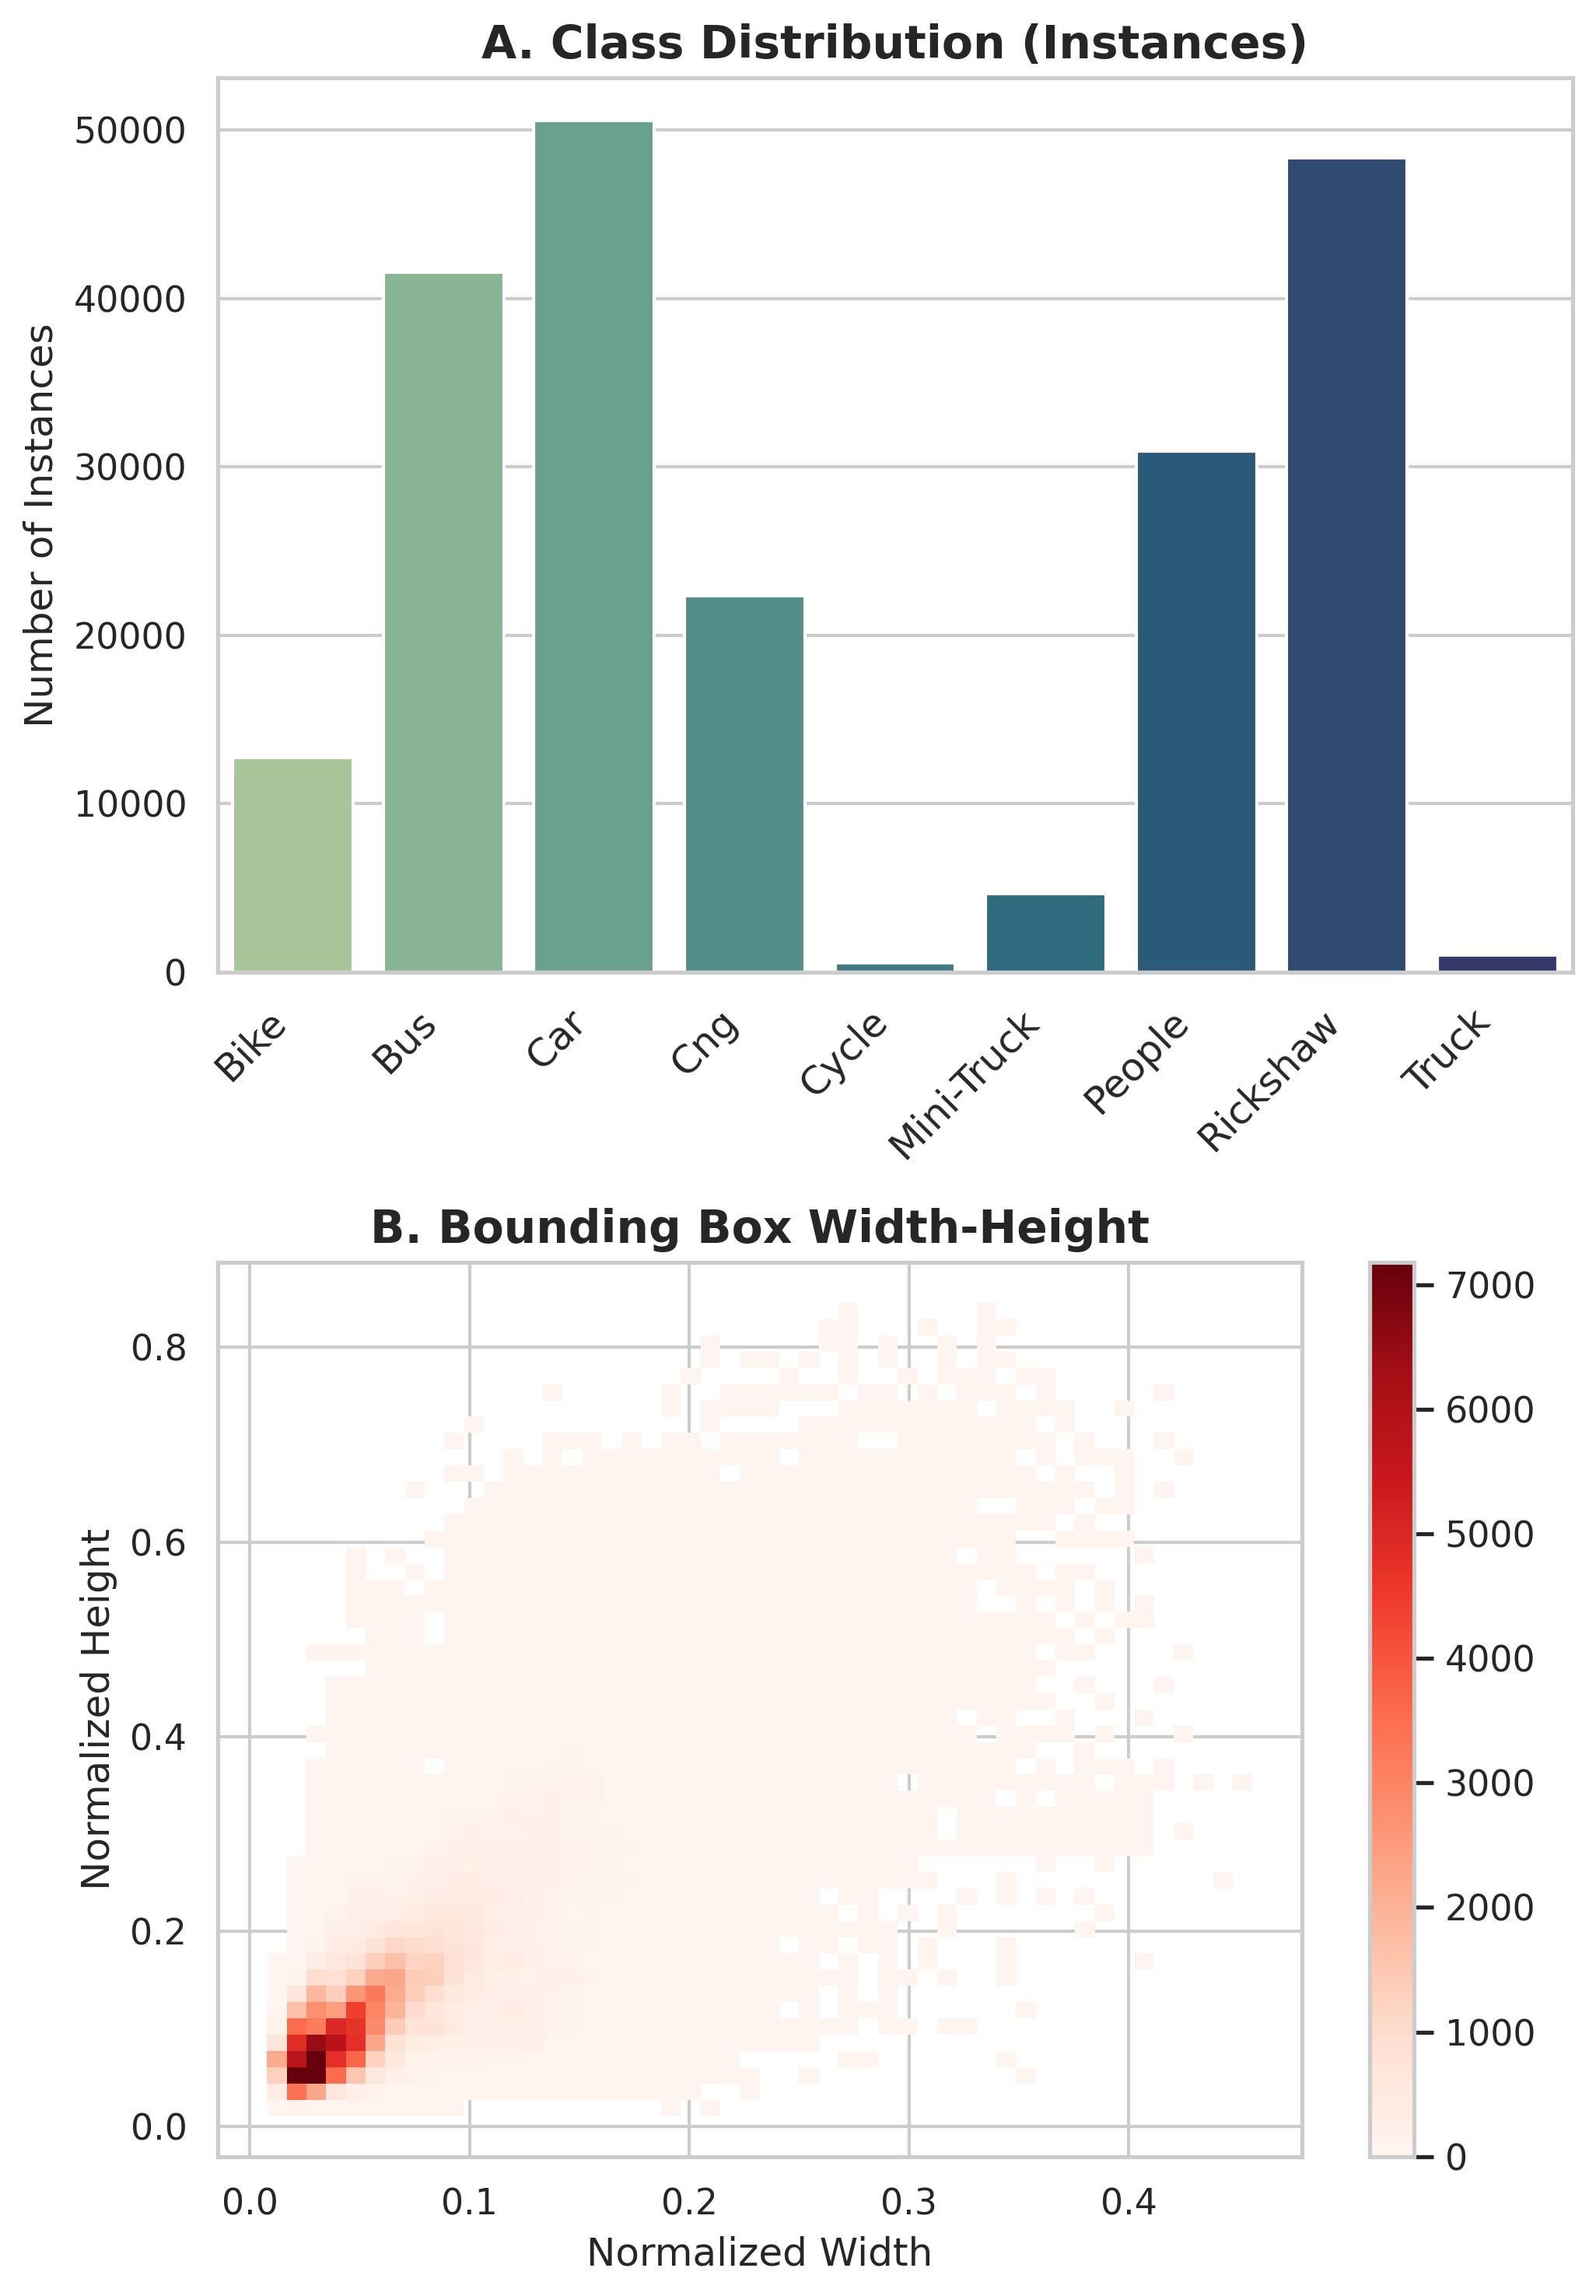
\includegraphics[width=\linewidth]{Images/IEEE_Single_Column_Stats.png}
\caption{Dataset statistics and bounding box characteristics of the finalized \texttt{masterv1} dataset (265,698 instances). (A) The class distribution illustrates a severe long-tailed imbalance, dominated by structurally similar local vehicles like Cars and Rickshaws. (B) The bounding box density distribution confirms that the vast majority of detections possess extremely small spatial dimensions, simulating the dense occlusion characteristic of unstructured Dhaka traffic.}
\label{fig:dataset_stats}
\end{figure}



\subsection{Advanced Augmentation Strategies}

Since the dataset contains a strong class imbalance, training the model with the original images alone can bias the model toward the dominant classes. To reduce this effect, we applied several data augmentation techniques during training using the Albumentations library. Specifically, we used Mosaic augmentation with a probability of 1.0, where four different images are combined into a single frame. This helps create crowded scenes and allows the model to learn from objects that are partially occluded. We applied an extra MixUp augmentation method that blends two images together with their corresponding labels. The MixUp approach helps the model to learn more stable features which reduces the chance of overfitting to dominant classes. 

\section{EXPERIMENTAL SETUP}

\subsection{Hardware and Configuration}

Baseline and modified models were trained with identical hyperparameters to ensure consistent evaluation and compared under the same setup for fairness. The models were trained in a cloud environment using NVIDIA T4 GPU with 16GB VRAM. 
\begin{table}[h]
\centering
\caption{Training Parameter Settings}
\label{tab:param}
\begin{tabular}{|c|l|l|}
\hline
\textbf{Sr. No.} & \textbf{Parameter} & \textbf{Value} \\ 
\hline
1 & Training Epochs & 50 \\ 
\hline
2 & Batch Size & 32 (distributed across dual \\ 
&&  GPUs)\\
\hline
3 & Optimizer & SGD (momentum = 0.937\\ 
&&  weight decay = 0.0005) \\
\hline
4 & Initial Learning Rate & 0.01 \\ 
\hline
5 & Learning Rate Scheduler & Cosine Annealing \\ 
\hline
6 & Input Resolution & 640 $\times$ 640 pixels \\ 
\hline
7 & Mixed Precision & Automatic Mixed Precision  \\ 

&&(AMP) Enabled\\
\hline
\end{tabular}
\end{table}

\subsection{Evaluation Metrics}This paper makes use of a better YOLOv11m architecture with a Convolutional Block Attention Module (CBAM) to further improve feature representation. It is experimentally shown that the initial YOLOv11m model achieves mAP of 75.1, and that the CBAM-based variant is more favorable in terms of detection performance.


\section{RESULTS AND ANALYSIS}
To evaluate the performance of our approach in dense traffic scenes, we carried out two experiments. First, a standard YOLOv11m model was trained from scratch on our custom dataset to establish a baseline for Bangladeshi traffic conditions. Although the baseline model performed reasonably well, we observed that it often struggled to separate bounding boxes when vehicles were very close to each other. To address this limitation, we then trained our modified YOLOv11m+CBAM model, which is designed to better handle occlusion in crowded traffic scenes.

\subsection{Quantitative Performance}
When fully trained across 50 epochs, both architectures demonstrated highly stable convergence. As shown in Table II, our initial baseline YOLOv11m achieved a strong 75.1\% mAP@50. However, the introduction of the attention mechanism in our second experiment successfully pushed the overall validation performance to 75.7\% mAP@50.

\begin{figure}[htbp]
\centering
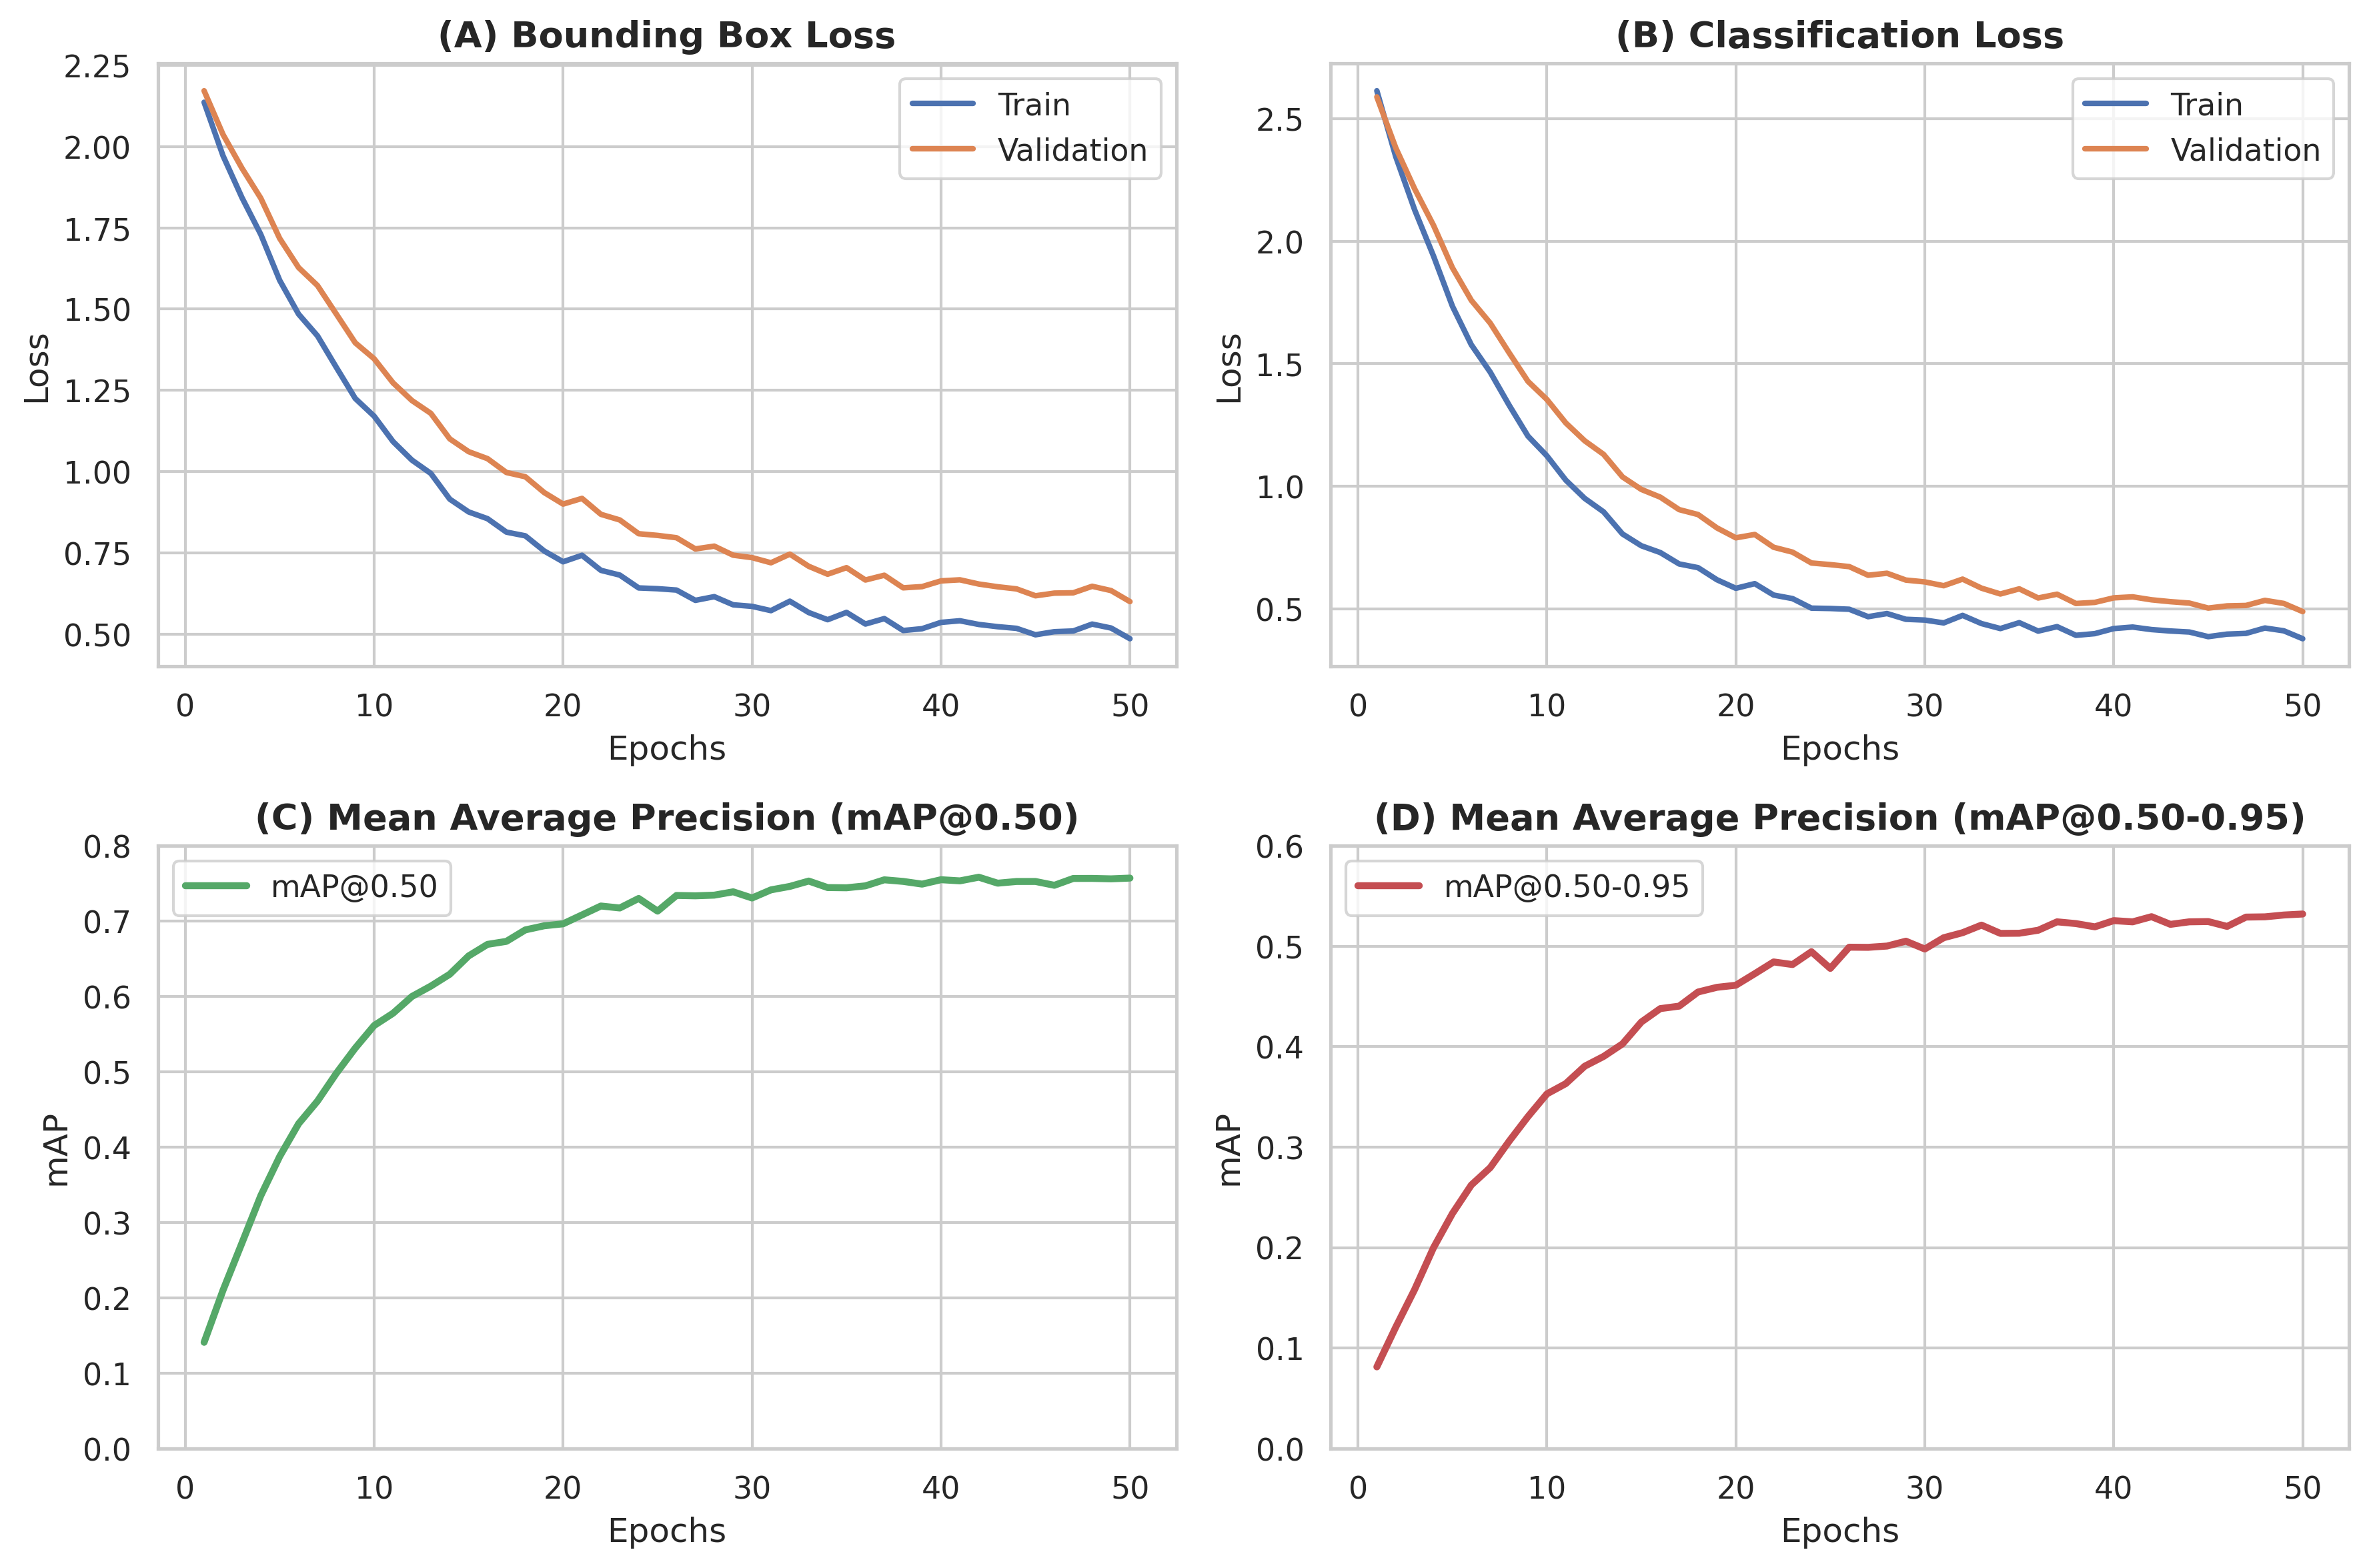
\includegraphics[width=\linewidth]{Images/training_curve_reconstructed.png}
\caption{Training and validation metrics across 50 epochs for the proposed YOLOv11m+CBAM architecture. (A) Bounding Box Loss and (B) Classification Loss demonstrate steady convergence, indicating the model localized and classified highly occluded vehicles without overfitting. (C) The primary mAP@0.50 metric and (D) the strict mAP@0.50--0.95 metric plateau efficiently, achieving final validation scores of 75.7\% and 53.2\%, respectively.}
\label{fig:training_curve}
\end{figure}


\begin{table}[htbp]
\caption{Ablation Study - Overall Performance}
\centering
\resizebox{\linewidth}{!}{%
\begin{tabular}{|c|c|c|c|c|}
\hline
\textbf{NO}
&\textbf{Architecture} & \textbf{mAP@0.5} & \textbf{ AP@0.5:0.95} & \textbf{Inference Speed} \\
\hline
Experiment & YOLOv11m baseline model& 0.751 & 0.528 & $\sim$5.0 ms \\ 

Experiment& YOLOv11m integrated with CBAM & 0.757 & 0.532 & $\sim$4.7 ms \\

\hline
\end{tabular}%
}
\label{tab:ablation_overall}
\end{table}


Breaking down the 75.7\% overall performance by class reveals a massive contrast in how the attention mechanism handles structurally distinct vehicles versus minority classes heavily impacted by the dataset's long-tailed imbalance.

\begin{table}[htbp]
\caption{Per-Class Average Precision (mAP@0.50)}
\centering
\resizebox{\linewidth}{!}{%
\begin{tabular}{|c|c|c|c|}
\hline
\textbf{Class Category} & \textbf{Vehicle Class} & \textbf{Baseline mAP@50} & \textbf{CBAM mAP@50} \\
\hline
{Dominant} 
 & Car       & 0.934 & 0.934 \\
 & CNG       & 0.910 & 0.911 \\
 & Rickshaw  & 0.905 & 0.908 \\
\hline
{Mid-Tier} 
 & Bus       & 0.892 & 0.894 \\
 & People    & 0.866 & 0.868 \\
 & Bike      & 0.837 & 0.846 \\
\hline
{Minority} 
 & Mini-Truck & 0.655 & 0.666 \\
 & Truck      & 0.455 & 0.470 \\
 & Cycle      & 0.305 & 0.316 \\
\hline
\end{tabular}%
}
\label{tab:per_class_map}
\end{table}

\begin{figure}[htbp]
\centering
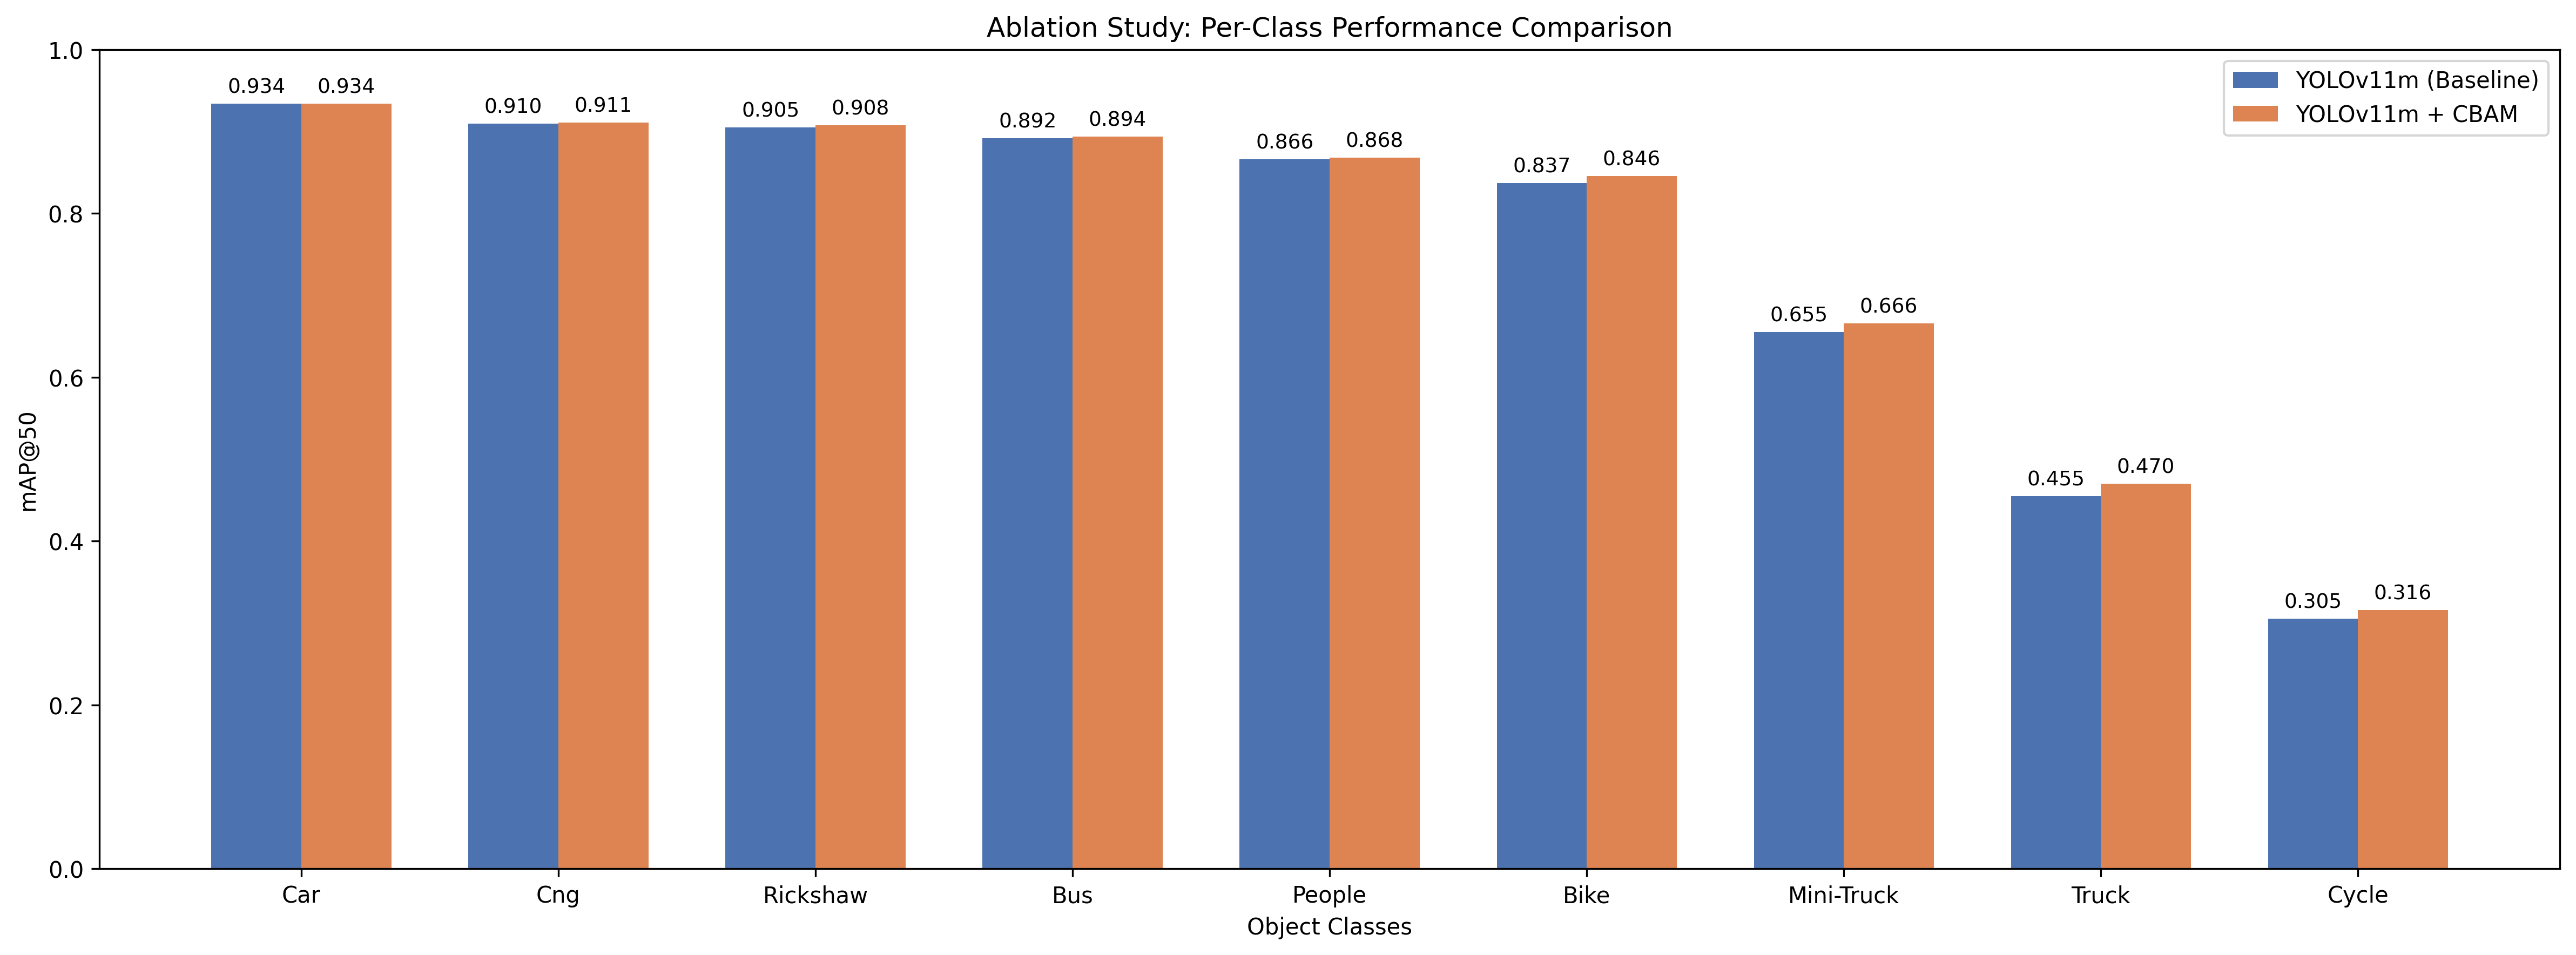
\includegraphics[width=\linewidth]{Images/ablation_study_map50.png}
\caption{Comparative study of per-class Average Precision (mAP@0.50). While our baseline model established strong initial metrics, the proposed YOLOv11m+CBAM architecture successfully extracted obscured features in heavily occluded minority classes, yielding significant accuracy boosts for Trucks (+1.5\%) and Mini-Trucks (+1.1\%).}
\label{fig:ablation_study_map50}
\end{figure}

The data confirms our hypothesis. For heavily represented classes like Cars, CNGs, and Rickshaws, the baseline model was already highly capable, pushing past 90\% accuracy. However, the standard convolutional layers failed on structurally distinct minority classes. By adding spatial and channel attention mechanisms, our second model provided massive accuracy boosts ($>1.0\%$) for Trucks, Mini-Trucks, and Cycles by mathematically forcing the network to parse heavy metallic textures.

\subsection{Computational Overhead}

A common drawback of adding attention modules is a loss of processing speed. To validate that our high accuracy was achieved without sacrificing operational viability, we benchmarked both of our models. Our initial baseline processed images at roughly 5.0ms per frame. Remarkably, our custom YOLOv11m+CBAM architecture maintained an exceptional 4.7ms inference speed on the Tesla T4. This proves that integrating CBAM deep within the backbone substantially boosts perception accuracy in heavy occlusion without introducing computational latency, perfectly preserving real-time capability for edge-device ADAS deployment.

\section{DISCUSSION AND ERROR ANALYSIS}
The YOLOv11m+CBAM model performs better in dense traffic scenes but many challenges remain including class imbalance, structural confusion between visually similar vehicles, and difficulties in detecting sparse or occluded objects. The following subsections issues each in detail.

\subsection{Class Imbalance and Detection Performance}

After training the model, it shows a clear pattern in the performance across different vehicle categories. The model performs very well on classes such as cars, rickshaws, buses, and CNGs, achieving high detection accuracy because of the high amount of data for these particular classes. On the other hand, the performance dropped significantly when identifying the minority classes, such as cycles and trucks. This indicates that the model is highly influenced by the distribution of training data. For better performance, it requires sufficient training of the model. The model achieves strong detection performance when only a large number of training samples are available for categories. Vehicles like cars, rickshaws, and buses appear frequently in the dataset, which allows the model to learn structural patterns more effectively. Additionally, these vehicles have distinct shapes and strong visual features, that's why it is easier for a convolutional neural network to detect them properly even in dense traffic areas. The model struggled to detect cycles because bicycles have very thin structural features. Another factor is dataset imbalance, as the number of cycle instances in the dataset is extremely low compared to other dominant classes. In many cases, the model focuses on the rider instead of the bicycle, which results in misclassification as a pedestrian.

\subsection{Structural Confusion Between Similar Vehicles}
Another issue appears for a similar geometric structure, confusion arises between buses and trucks which makes them visually difficult to separate. Since the dataset contains far fewer truck as a result, trucks are frequently misclassified as buses. As shown in Fig.~\ref{fig:confusion_matrix}, the confusion shown inside the normalized confusion matrix where some truck instances are predicted as buses. This indicates that the model depends mostly on the dominant class during classification when distinctive features are not clearly visible. The dataset follows a long-tailed distribution where dominant classes have thousands of instances, but minority classes contain only a few hundred samples. This imbalance highly affects the learning process, the model received much more training feedback from dominant classes. Consequently, the model becomes biased towards these dominant classes and predicts them correctly, but struggles to correctly identify the minority classes. This often leads to higher false negative rates for minority classes and misclassification errors during inference.


\begin{figure}[htbp]
\centering
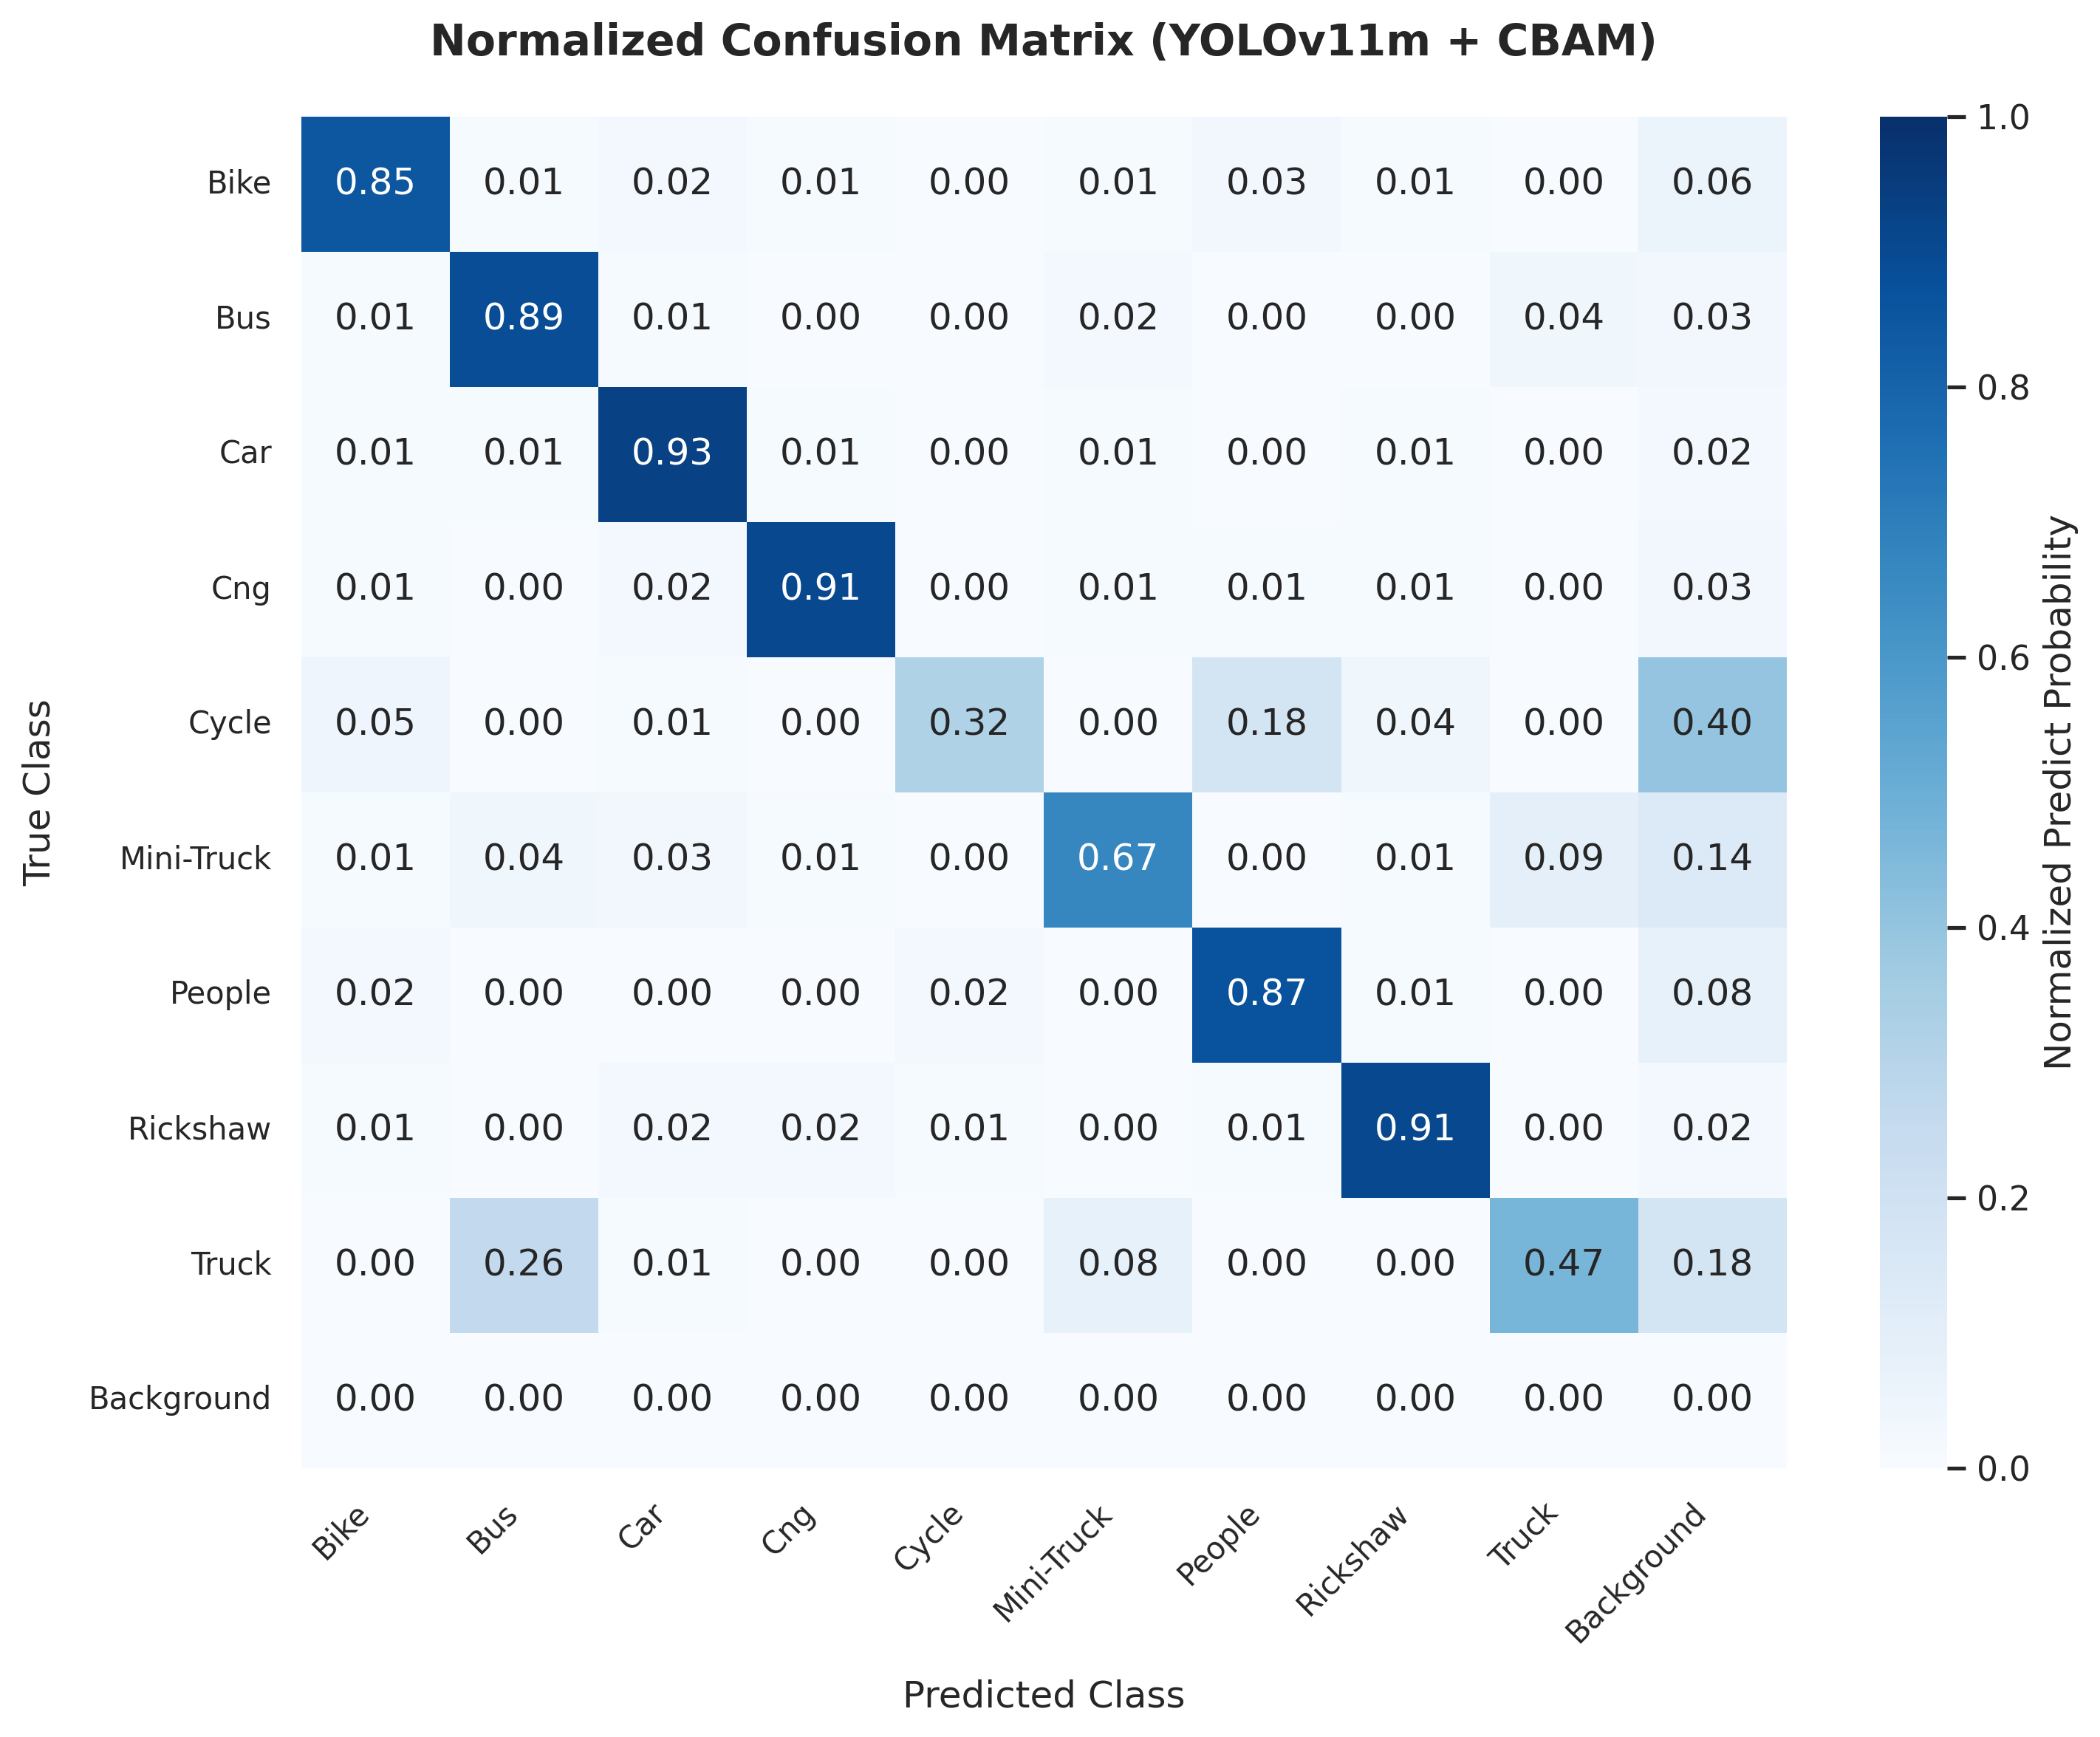
\includegraphics[width=\linewidth]{Images/confusion_matrix_reconstructed.png}
\caption{Normalized confusion matrix of YOLOv11m+CBAM showing false negatives for the Cycle class and notable cross-confusion among large vehicle classes.}
\label{fig:confusion_matrix}
\end{figure}

\subsection{Qualitative Performance}

We checked predictions from the validation dataset to better understand the model behavior. As shown in Fig.~\ref{fig:qualitative_results} the architecture produces tight and well-separated bounding boxes, even in dense traffic. In crowded scenes, the detector correctly identifies overlapping vehicles like cars, rickshaws and buses. By integrating CBAM attention module helps the network to focus on spatial and channel features, reducing suppression issues and improves consistent detection in complex environments, especially with occlusion and clutter.

\begin{figure}[htbp]
\centering
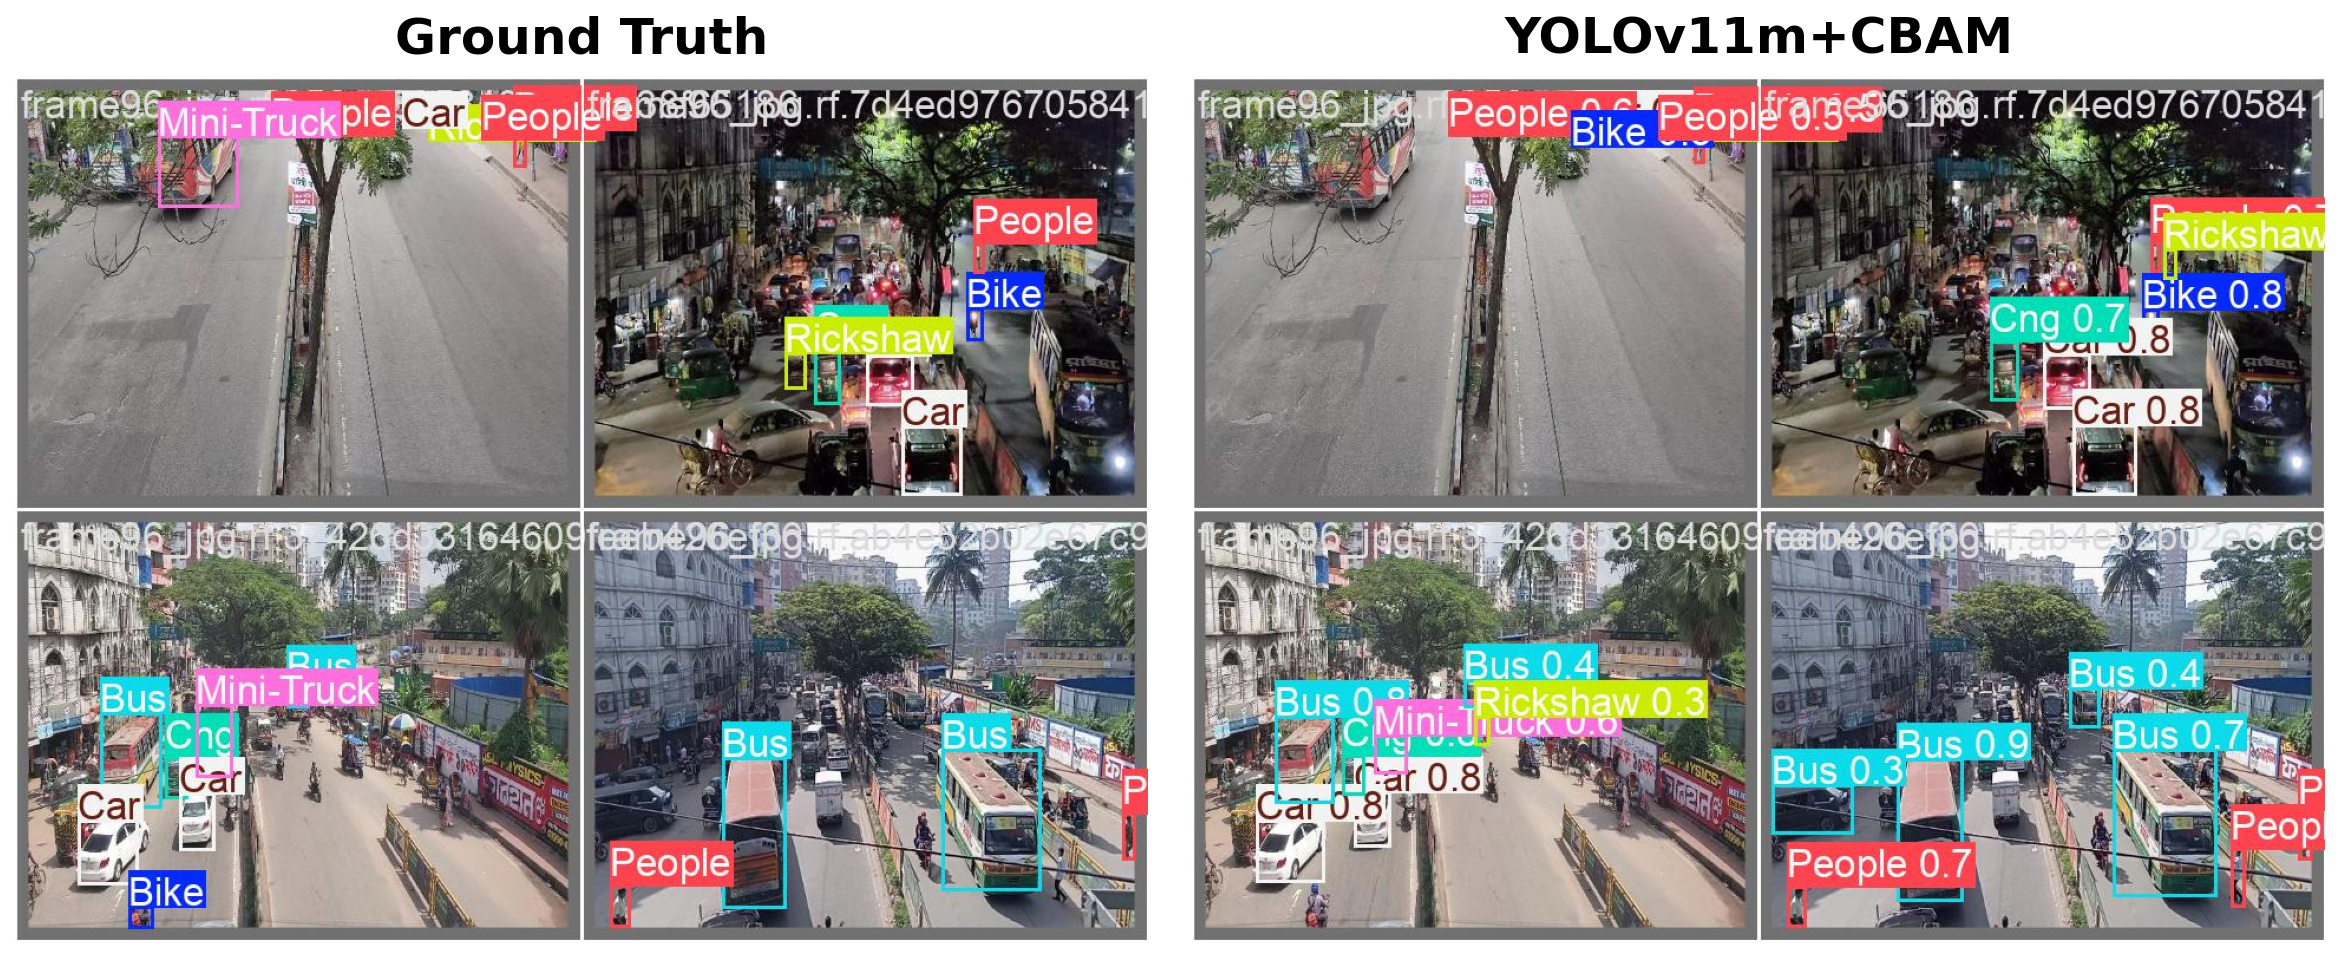
\includegraphics[width=\linewidth]{Images/IEEE_Qualitative_Results.png}
\caption{Qualitative detection results on the validation set. Left: ground truth annotations. Right: predictions from the YOLOv11m+CBAM model in dense unstructured traffic.}
\label{fig:qualitative_results}
\end{figure}

However, the qualitative results also reveal limitations and some challenges still remain. The model still struggles with sparse structural objects such as cycles, especially when only a limited number of training samples are available. In addition, vehicles with similar visual structures, such as trucks and buses, remain difficult to distinguish when their visual features appear very similar. These observations indicate that architectural improvements alone may not fully solve the problem. Future work should therefore focus on improving dataset balance and collecting more samples for minority vehicle classes.

\section{CONCLUSION AND FUTURE WORK}
The main objective of this research was to improve object detection in unstructured Bangladeshi traffic environments, we develop a modified detection model. A large unified dataset of Bangladesh was created by merging multiple region-based datasets. For improving feature extraction in dense and occluded traffic scenes, a modified Yolov11m  architecture and a Convolution Block Attention model are integrated. The experimental results showed that the baseline model achieved 75.1\% mAP, while the proposed attention model, Yolov11 + CBAM model, improved performance to 75.7\% mAP. The model performs better on local vehicle Classes such as Rickshaws and CNGs, achieving detection accuracy above 90\%. These results are significant for Intelligent Transportation Systems (ITS) and Advanced Driver Assistance Systems (ADAS) in developing countries. which  improve road safety, traffic monitoring, and autonomous driving technology. Aside from these  the model still faces limitations due to several class imbalances. For minority classes, such as cycles and trucks. Future research will focus on the dataset imbalance problem. 








\bibliographystyle{IEEEtran}
\bibliography{rf}


\end{document}
